\subsubsection{Дисперсионная схема дифракции}
\begin{figure}[h]
  \centering
  \subfloat[Образец Si(440), $S_1 = S_2 = 100$ мкм.]{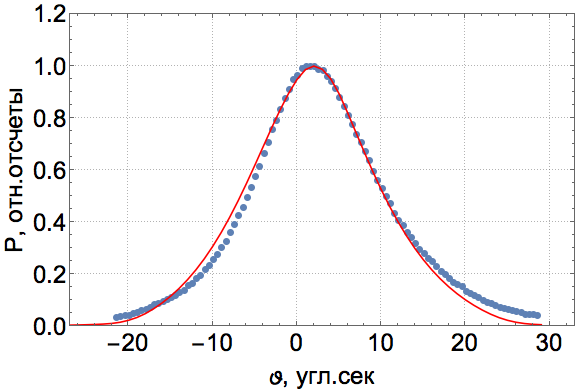
\includegraphics[width=0.45\textwidth]{images/disspers_220_440_100mcm.png}\label{fig:f1}}
  \hfill
  \subfloat[Образец Si(660), $S_1 = S_2 = 100$ мкм.]{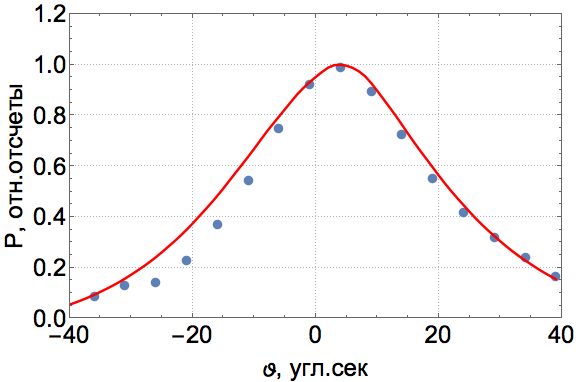
\includegraphics[width=0.45\textwidth]{images/disspers_220_660_100mcm.png}\label{fig:f2}}
  \hfill
  \subfloat[Образец Si(440), $S_1 = S_2 = 300$ мкм.]{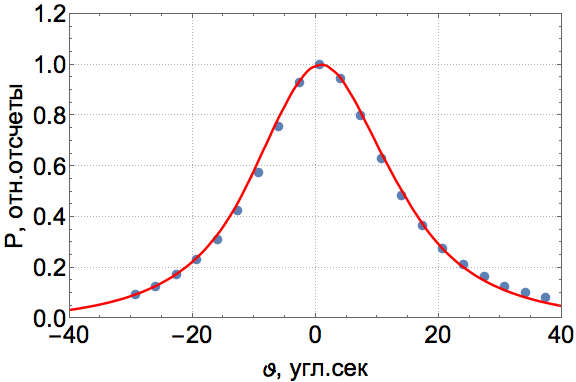
\includegraphics[width=0.45\textwidth]{images/disspers_220_440_300mcm.png}\label{fig:f2}}
  \hfill
  \subfloat[Образец Si(660), $S_1 = S_2 = 300$ мкм.]{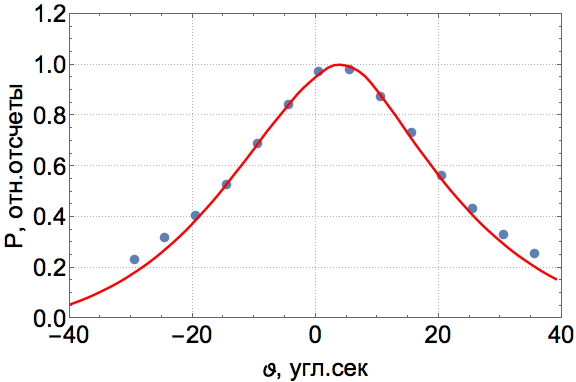
\includegraphics[width=0.45\textwidth]{images/disspers_220_660_300mcm.png}\label{fig:f2}}
  \caption{Двухкристальная КДО для схемы с кристаллом монохроматором Si(220) для дисперсионного случая}
  \label{ris:disspersion_curves_expantheory}
\end{figure}
